\svnidlong{$HeadURL: https://www.fontysvenlo.org/svnp/879417/latexcolloquium/trunk/latexsample/graphics.tex $}%
{$LastChangedDate: 2014-02-23 19:48:59 +0100 (Sun, 23 Feb 2014) $}%
{$LastChangedRevision: 55 $}%
{$LastChangedBy: 879417 $}
\svnid{$Id: graphics.tex 55 2014-02-23 18:48:59Z 879417 $}
\renewcommand\TheFile{graphics.tex}
\begin{savequote}[6cm]
  \sffamily
A picture is worth 1000 words
  \qauthor{Anonymous}
\end{savequote}
\chapter{Graphics as easy as pie}
\LaTeX, combined with pdf in \texttt{pdflatex}, supports the following
graphic file types: pdf, png, jpeg or jpg and gif in that order of
preference. Using the vector format pdf gives the added benefit that
the graphic file can be scaled up and down without loss of quality.
If you want to include bitmaps, try to get them in png format which
is open and patent free. It has the advantage over jpeg or jpg that is is
loss-less, so you do not see any artifact if you blow them up in your
inclusion. Converting back from jpg to png is useless, because the
damage is already done in the jpeg format. JPEG is excellent for
photographs. For all the bitmap formats: try to get them at the
intended size with a resolution of 300dpi for printouts. 75 dpi is
acceptable for screen reading.
  
\begin{figure}[thbp]
  \centering
  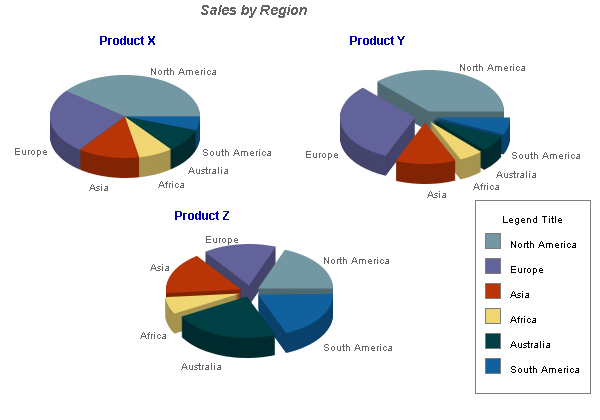
\includegraphics[width=.8\textwidth]{figures/servlet3.png}
  \caption[A Pie chart]{Stolen from the net. Google for a pie chart...}
  \label{fig:pie}
\end{figure}

Many graphics packages can produce pdf files
Embedded postscript (file extension .eps) are also a good candidate,
after converting them to pdf with the epstopdf tool. By the way: the
native format of Adobe Illustrator (ai) is similar enough to eps, so
that too can be processed with ps2pdf. Programs like {\em Visual
  Paradigm} are able to produce pdf files too. And sometimes open-office can
lend a helping hand, for by cutting and pasting Windows graphics into
a single page oodraw drawing, you can produce an very usable pdf file. 

Bitmap file types like png and jpeg take up a lot of space in your
final pdf document. 
Bitmap files take even more space if encoded into a pdf file.
If at all possible, stick to a vector format like eps or pdf (if
necessary derived from eps files). 

%\clearpage%to show headers

\section{A png example}
\label{page:pngexample}
If latex cannot fit the diagram on this page
(page~\pageref{page:pngexample}), 
 then you may find the diagram as figure~\vref{fig:pie}. And as you
 can see, you can easily reference pages and figures.

%\clearpage%to show headers
\section{PDF from an UML package} 
% Note how this varioref expands to
% something like on the next page.
% and using a wrapfigure
\begin{wrapfigure}{r}{.4\textwidth}

  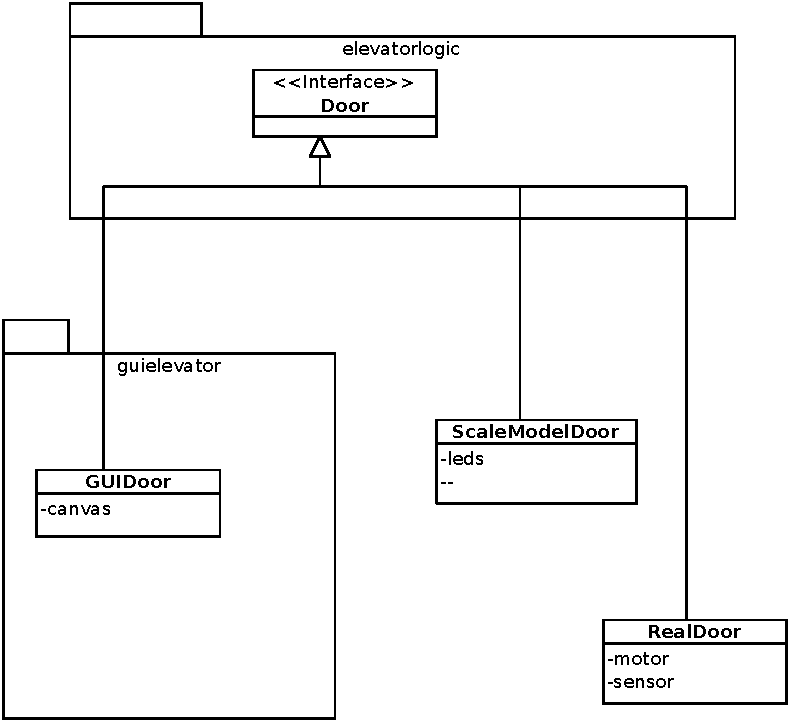
\includegraphics[width=.4\textwidth]{figures/doorsystem.pdf}
  \caption{A class diagram made with Visual Paradigm}
  \label{fig:classdiagram}
\end{wrapfigure}
If the documentation you write is a design document of some software
package, you may want to include design diagrams.
No software engineering without a UML diagrams\ldots.
You can see one generated with ``dia'', a vector drawing program that
understands the UML in figure~\ref{fig:classdiagram}
~\vpageref{fig:classdiagram}. This diagram is 'wrapped' in a \Code{wrapfigure} environment, so the text may flow around it

The diagram is not very sophisticated but shows an example of a vector
format file included via an eps$\rightarrow$ pdf conversion by
epstopdf.

Open source programs like umlet and argouml are also able to produce
vector format graphics files. And sometimes it is helpful to add a box 
that is a bit bigger then the picture you want to include.
This ensures that the so called bounding box does not cut of any lines
you want in your picture. Sometimes it is necessary to give these
tools a helping hand with inkscape, that is do a bit of tinkering to
get all details right.
\begin{figure}[htbp]
  \centering
  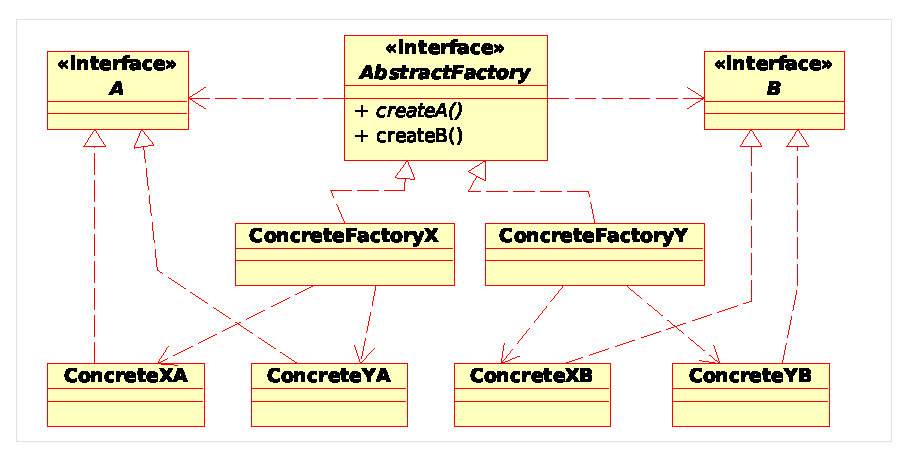
\includegraphics[width=.6\textwidth]{figures/factory}
  \caption[A class diagram by Umbrello]{A class diagram by Umbrello, saved as svg and processed
    with inkscape.}
  \label{fig:factory}
\end{figure}

% On the front cover you can find an ArgoUml diagram that shows how you could
% arrange a set of files, which would allow you to present on screen or on
% paper and in several languages from the same source files. We use this
% to prepare our freshmen syllabi and exams.

%%% Local Variables: 
%%% mode: latex
%%% TeX-master: "main"
%%% End: 
